\documentclass[border=10pt]{standalone}
\usepackage[T1]{fontenc}\usepackage[utf8]{inputenc}\usepackage{lmodern}
\usepackage{tikz}\usetikzlibrary{arrows.meta,positioning,calc}
\begin{document}
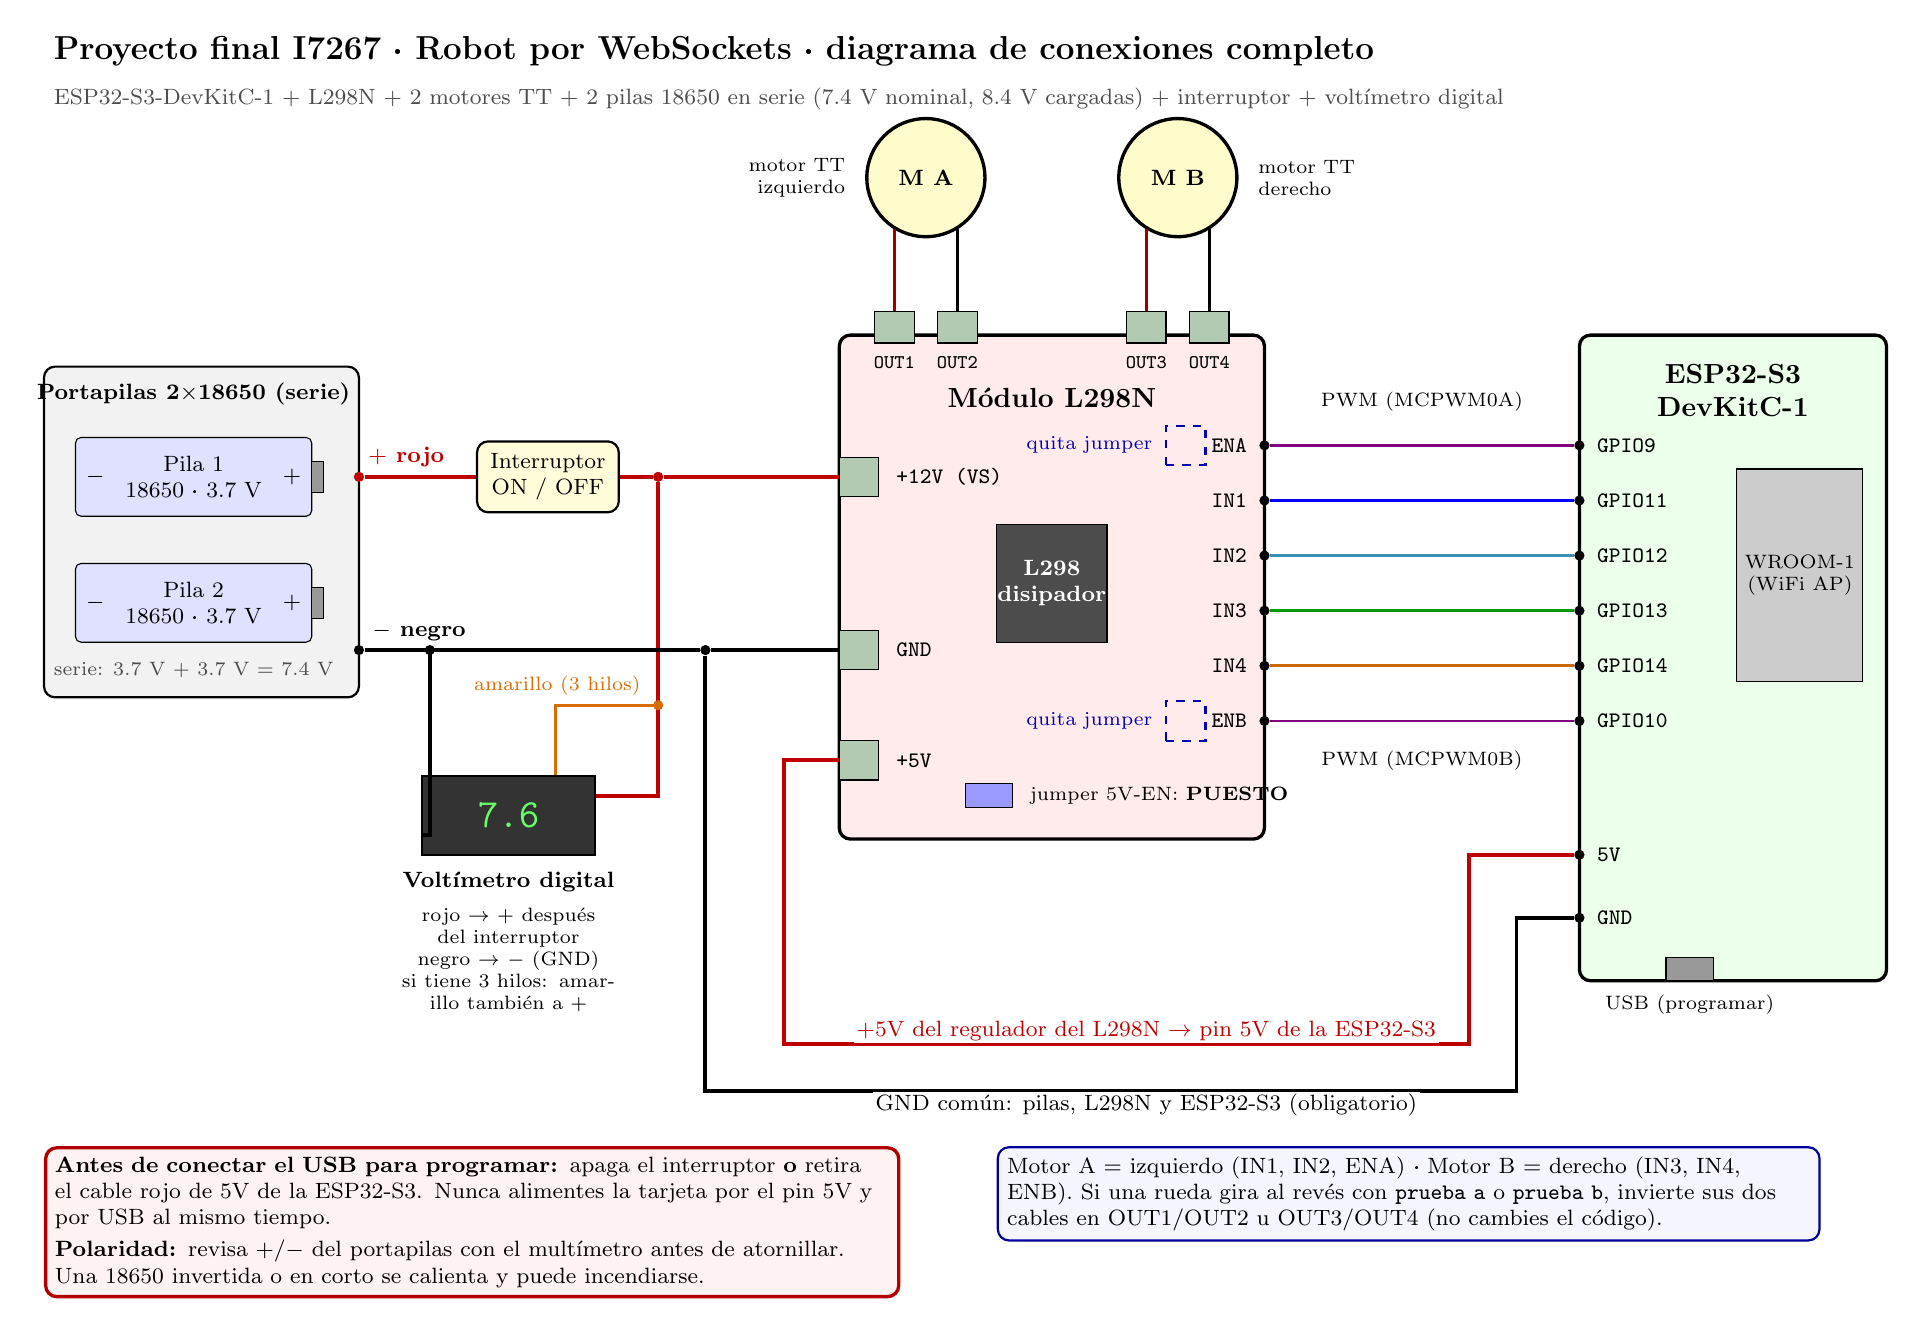
\begin{tikzpicture}[>=Latex,font=\small,
  pin/.style={font=\footnotesize\ttfamily},
  rojo/.style={draw=red!75!black,line width=1.4pt},
  negro/.style={draw=black,line width=1.4pt},
  amar/.style={draw=orange!85!black,line width=1.1pt},
  sen/.style={line width=1.0pt},
  pt/.style={circle,fill,inner sep=1.3pt}]

% ------------------------------------------------ Titulo
\node[font=\large\bfseries,anchor=west] at (-0.5,14.6) {Proyecto final I7267 · Robot por WebSockets · diagrama de conexiones completo};
\node[font=\footnotesize,anchor=west,text=black!70] at (-0.5,14.0) {ESP32-S3-DevKitC-1 + L298N + 2 motores TT + 2 pilas 18650 en serie (7.4 V nominal, 8.4 V cargadas) + interruptor + voltímetro digital};

% ------------------------------------------------ Portapilas 2x18650
\draw[thick,fill=black!5,rounded corners] (-0.5,6.4) rectangle (3.5,10.6);
\node[font=\bfseries\footnotesize] at (1.4,10.25) {Portapilas 2$\times$18650 (serie)};
\foreach \y/\t in {9.2/Pila 1, 7.6/Pila 2}{
  \draw[fill=blue!12,rounded corners=2pt] (-0.1,\y-0.5) rectangle (2.9,\y+0.5);
  \draw[fill=black!40] (2.9,\y-0.2) rectangle (3.05,\y+0.2);
  \node[font=\footnotesize,align=center] at (1.4,\y) {\t\\18650 · 3.7 V};
  \node[font=\footnotesize\bfseries] at (2.65,\y) {$+$};
  \node[font=\footnotesize\bfseries] at (0.15,\y) {$-$};
}
\node[font=\scriptsize,text=black!70] at (1.4,6.75) {serie: 3.7 V + 3.7 V = 7.4 V};
\node[pt,red!75!black] (bp) at (3.5,9.2) {};
\node[pt] (bn) at (3.5,7.0) {};
\node[font=\footnotesize\bfseries,red!75!black,anchor=south west] at (3.5,9.2) {$+$ rojo};
\node[font=\footnotesize\bfseries,anchor=south west] at (3.55,7.0) {$-$ negro};

% ------------------------------------------------ Interruptor
\node[draw,thick,fill=yellow!15,rounded corners,minimum width=1.8cm,minimum height=0.9cm,align=center,font=\footnotesize] (sw) at (5.9,9.2) {Interruptor\\ON / OFF};
\draw[rojo] (bp) -- (sw.west);

% ------------------------------------------------ Voltimetro
\node[draw,thick,fill=black!80,text=green!60,minimum width=2.2cm,minimum height=1.0cm,font=\Large\ttfamily\bfseries] (vm) at (5.4,4.9) {7.6};
\node[font=\footnotesize\bfseries,anchor=north] at (5.4,4.3) {Voltímetro digital};
\node[font=\scriptsize,align=center,anchor=north,text width=3.8cm] at (5.4,3.85) {rojo $\to$ $+$ después del interruptor\\negro $\to$ $-$ (GND)\\si tiene 3 hilos: amarillo también a $+$};
\node[pt,red!75!black] (j1) at (7.3,9.2) {};
\draw[rojo] (sw.east) -- (j1);
\draw[rojo] (j1) |- ($(vm.east)+(0,0.25)$);
\draw[amar] ($(j1)+(0,-2.9)$) node[pt,orange!85!black]{} -| ($(vm.north)+(0.6,0)$);
\node[font=\scriptsize,orange!85!black,anchor=south east] at (7.2,6.3) {amarillo (3 hilos)};
\node[pt] (j2) at (7.9,7.0) {};
\draw[negro] (bn) -- (j2);
\draw[negro] ($(bn)+(0.9,0)$) node[pt]{} |- ($(vm.west)+(0,-0.25)$);

% ------------------------------------------------ L298N
\draw[very thick,fill=red!8,rounded corners] (9.6,4.6) rectangle (15.0,11.0);
\node[font=\bfseries] at (12.3,10.2) {Módulo L298N};
\draw[fill=black!70] (11.6,7.1) rectangle (13.0,8.6);
\node[text=white,font=\footnotesize\bfseries,align=center] at (12.3,7.85) {L298\\disipador};
% bornera de potencia (izquierda)
\foreach \y/\t in {9.2/+12V (VS), 7.0/GND, 5.6/+5V}{
  \draw[fill=green!30!black!30] (9.6,\y-0.25) rectangle (10.1,\y+0.25);
  \node[pin,anchor=west] at (10.2,\y) {\t};
}
% jumper 5V-EN
\draw[fill=blue!40] (11.2,5.0) rectangle (11.8,5.3);
\node[font=\scriptsize,anchor=west,align=left] at (11.9,5.15) {jumper 5V-EN: \textbf{PUESTO}};
% salidas a motores (arriba)
\foreach \x/\t in {10.3/OUT1, 11.1/OUT2, 13.5/OUT3, 14.3/OUT4}{
  \draw[fill=green!30!black!30] (\x-0.25,10.9) rectangle (\x+0.25,11.3);
  \node[pin,font=\scriptsize\ttfamily,anchor=north] at (\x,10.85) {\t};
}
% cabecera de control (derecha)
\foreach \y/\t in {9.6/ENA, 8.9/IN1, 8.2/IN2, 7.5/IN3, 6.8/IN4, 6.1/ENB}{
  \node[pt] (L\t) at (15.0,\y) {};
  \node[pin,anchor=east] at (14.9,\y) {\t};
}
\draw[dashed,thick,blue!70!black] (13.75,9.35) rectangle (14.25,9.85);
\draw[dashed,thick,blue!70!black] (13.75,5.85) rectangle (14.25,6.35);
\node[font=\scriptsize,blue!70!black,anchor=east] at (13.7,6.1) {quita jumper};
\node[font=\scriptsize,blue!70!black,anchor=east] at (13.7,9.6) {quita jumper};

% potencia hacia la bornera
\draw[rojo] (j1) -- (9.6,9.2);
\draw[negro] (j2) -- (9.6,7.0);

% ------------------------------------------------ Motores
\node[draw,very thick,circle,minimum size=1.5cm,fill=yellow!20,align=center,font=\footnotesize\bfseries] (ma) at (10.7,13.0) {M A};
\node[draw,very thick,circle,minimum size=1.5cm,fill=yellow!20,align=center,font=\footnotesize\bfseries] (mb) at (13.9,13.0) {M B};
\node[font=\scriptsize,anchor=east,align=right] at (9.8,13.0) {motor TT\\izquierdo};
\node[font=\scriptsize,anchor=west,align=left] at (14.8,13.0) {motor TT\\derecho};
\draw[sen,draw=red!60!black] (10.3,11.3) -- (10.3,12.35);
\draw[sen] (11.1,11.3) -- (11.1,12.35);
\draw[sen,draw=red!60!black] (13.5,11.3) -- (13.5,12.35);
\draw[sen] (14.3,11.3) -- (14.3,12.35);

% ------------------------------------------------ ESP32-S3
\draw[very thick,fill=green!8,rounded corners] (19.0,2.8) rectangle (22.9,11.0);
\node[font=\bfseries,align=center] at (20.95,10.3) {ESP32-S3\\DevKitC-1};
\draw[fill=black!20] (21.0,6.6) rectangle (22.6,9.3);
\node[font=\scriptsize,align=center] at (21.8,7.95) {WROOM-1\\(WiFi AP)};
\foreach \y/\t in {9.6/GPIO9, 8.9/GPIO11, 8.2/GPIO12, 7.5/GPIO13, 6.8/GPIO14, 6.1/GPIO10, 4.4/5V, 3.6/GND}{
  \node[pt] (E\t) at (19.0,\y) {};
  \node[pin,anchor=west] at (19.1,\y) {\t};
}
\draw[fill=black!40] (20.1,2.8) rectangle (20.7,3.1);
\node[font=\scriptsize,anchor=north] at (20.4,2.75) {USB (programar)};

% senales de control
\foreach \a/\b/\c in {ENA/GPIO9/violet, IN1/GPIO11/blue, IN2/GPIO12/cyan!70!black, IN3/GPIO13/green!60!black, IN4/GPIO14/orange!80!black, ENB/GPIO10/violet}{
  \draw[sen,draw=\c] (L\a) -- (E\b);
}
\node[font=\scriptsize,align=center,fill=white,inner sep=1pt] at (17.0,10.15) {PWM (MCPWM0A)};
\node[font=\scriptsize,align=center,fill=white,inner sep=1pt] at (17.0,5.6) {PWM (MCPWM0B)};

% 5V y GND hacia la ESP32
\draw[rojo] (9.6,5.6) -- (8.9,5.6) |- (17.6,2.0) |- (E5V);
\draw[negro] (j2) |- (18.2,1.4) |- (EGND);
\node[font=\footnotesize,red!75!black,anchor=south,fill=white,inner sep=1pt] at (13.5,2.0) {+5V del regulador del L298N $\to$ pin 5V de la ESP32-S3};
\node[font=\footnotesize,anchor=north,fill=white,inner sep=1pt] at (13.5,1.4) {GND común: pilas, L298N y ESP32-S3 (obligatorio)};

% ------------------------------------------------ Avisos
\node[draw=red!70!black,very thick,fill=red!5,rounded corners,text width=10.6cm,align=left,font=\footnotesize,anchor=north west] at (-0.5,0.7) {%
\textbf{Antes de conectar el USB para programar:} apaga el interruptor \textbf{o} retira el cable rojo de 5V de la ESP32-S3. Nunca alimentes la tarjeta por el pin 5V y por USB al mismo tiempo.\\[2pt]
\textbf{Polaridad:} revisa $+$/$-$ del portapilas con el multímetro antes de atornillar. Una 18650 invertida o en corto se calienta y puede incendiarse.};
\node[draw=blue!60!black,thick,fill=blue!4,rounded corners,text width=10.2cm,align=left,font=\footnotesize,anchor=north west] at (11.6,0.7) {%
Motor A = izquierdo (IN1, IN2, ENA) · Motor B = derecho (IN3, IN4, ENB). Si una rueda gira al revés con \texttt{prueba a} o \texttt{prueba b}, invierte sus dos cables en OUT1/OUT2 u OUT3/OUT4 (no cambies el código).};
\end{tikzpicture}
\end{document}
